\documentclass[a4paper,12pt]{article}
\usepackage{graphicx, geometry, subfigure, amsmath, adjustbox, array}
\geometry{a4paper,left=2cm,right=2cm,top=1cm,bottom=2cm}
\setlength{\baselineskip}{12pt}
\renewcommand\arraystretch{1.5}

\title{\textbf{Stars and Planets Problem Set \uppercase\expandafter{\romannumeral1}}}
\author{Qingru Hu}
\date{\today}

\begin{document}
\maketitle

\section*{\textbf{Exercise \uppercase\expandafter{\romannumeral1}.1 Sun's efficiency}}
We can calculate the energy density of the Sun from the 
solar constant, that is the energy recieved by the Earth surface in 
unit area in unit time. 
The solar constant is $P = 1362 \ \text{W} \text{m}^{-2}$, and we know that 
the distance from the Sun to the Earth is $r = 1$ au, so we 
can calculate the luminosity of the Sun:
\begin{equation}
    L = 4 \pi r^2 P = 3.83 \times 10^{26} \ W
\end{equation}
Therefore, the energy output of the Sun per unit mass $\rho_\text{E, Sun}$ is:
\begin{equation}
    \rho_\text{E, Sun} = \frac{L}{M_{\bigodot}} = 1.92 \times 10^{-4} \ \text{W} \ \text{kg}^{-1}
\end{equation}

The radiation energy density of a human being can be 
estimated from a human being's body temperature, which is normally $T = 310 \ K$.
And we can assume that the skin area of a human being is about $A=0.5 \ m^2$, and 
the mass of a human being is $m = 50 \ \text{kg}$.
If we assume that the radiation of a human being obey the blackbody radiation, 
we can calculate the radiation energy density $\rho_{\text{E, Human}}$ of a human being to be:
\begin{equation}
    \rho_\text{E, Human} = \frac{\sigma T^4 A}{m} = 5.236 \ W \ \text{kg}^{-1}
\end{equation}

\section*{\textbf{Exercise \uppercase\expandafter{\romannumeral1}.2 Color-Magnitude diagram}}
\subsection*{(a)}
I choose the "hipparcos-bright.txt" dataset to draw the 
color-magnitude diagram Fig.\ref{fig1}. The star that has the greatest parallax is 
highlighted with a blue dot and the brightest one with a red dot.
\begin{figure}[htbp]
    \centering
    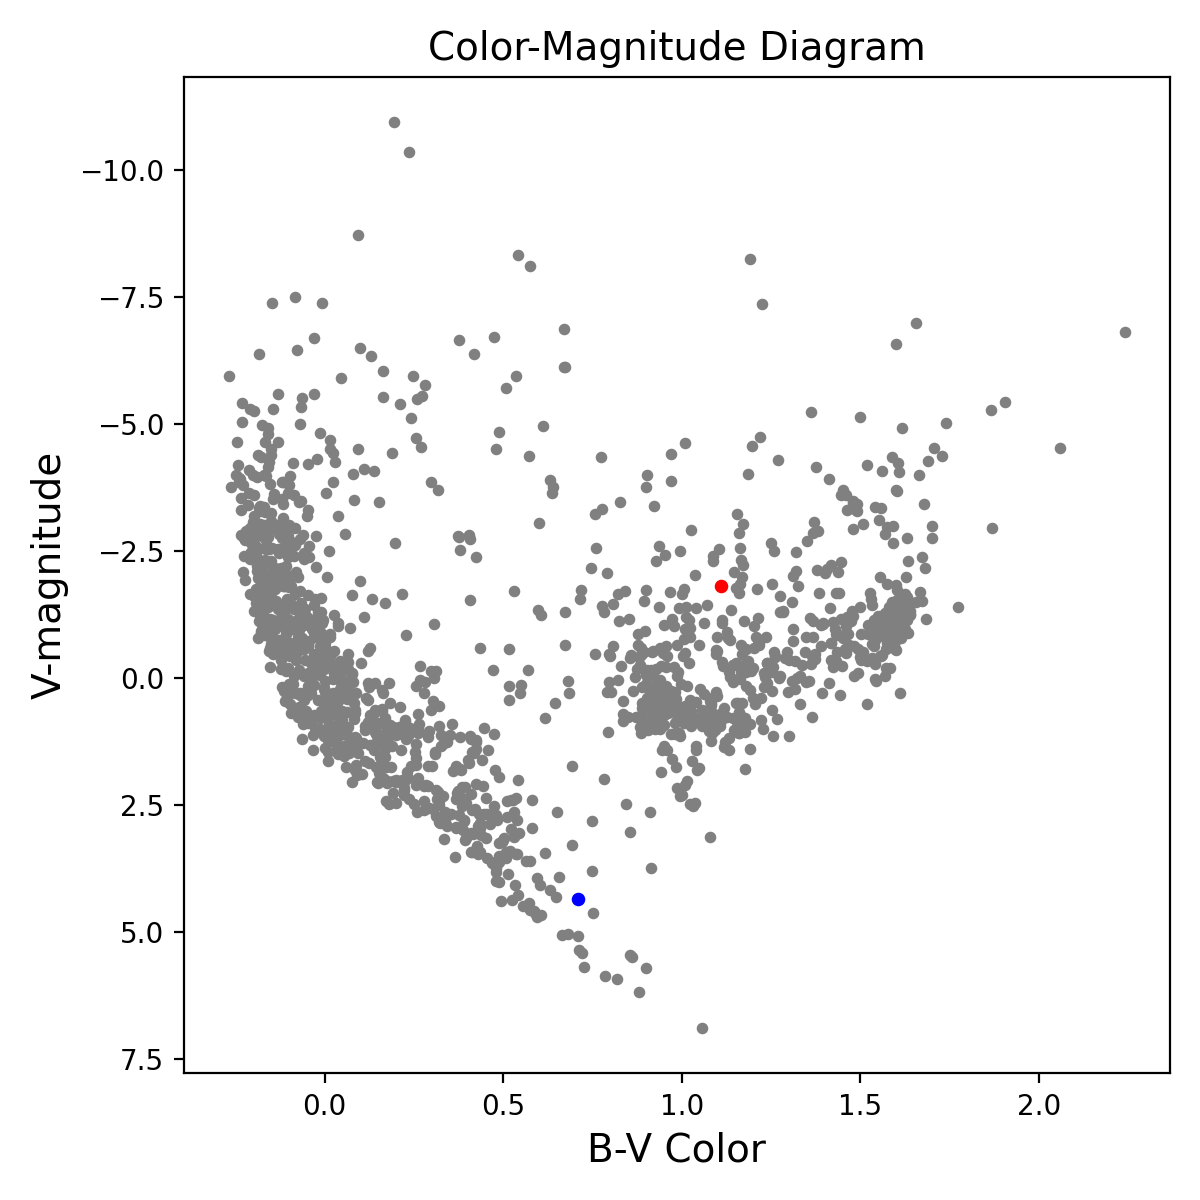
\includegraphics[width=8cm]{color_mag.png}
    \caption{The color-magnitude diagram of ``hipparcos-bright.txt"}
    \label{fig1}
\end{figure}

\subsection*{(b)}
That's because for a specific star the apparent and the absolute 
differ only by a constant.
\begin{equation}
    m-M = 5 \text{log}_{10}(\frac{d}{10pc})
\end{equation}
The $B-V$ color index is defined as 
the subtraction of magnitudes at the $B$ and $V$ bands, so the constant 
cancels out.

\subsection*{(c)}
According to the Wien's displacement law:
\begin{equation}
    \lambda_{\text{max}} = \frac{0.2898 \ \text{cm} \ \text{K}}{T}
\end{equation}
the higher the effective temperature $T_{\text{eff}}$, 
the shorter the wavelength of the maximum radiation will be.
The flux in both bands will increase, but it will increae more 
in the "blue" band (B). 
Therefore, the magnitude of the star will decrease more in the ``blue" band (B) 
and less in the ``visual" band (V), and their subtraction $B-V$ 
color is lower. 
That's why stars of higher $B-V$ have lower $T_{\text{eff}}$.

\subsection*{(d)}
The ``hipparcos-bright" sample doesn't contain white dwarfs. The main sequence 
stars and the RGB stars are labeled as 
blue and orange respectively in the Fig.\ref{class}. 
I only does a rough classification of these two groups of stars.
\begin{figure}[htbp]
    \centering
    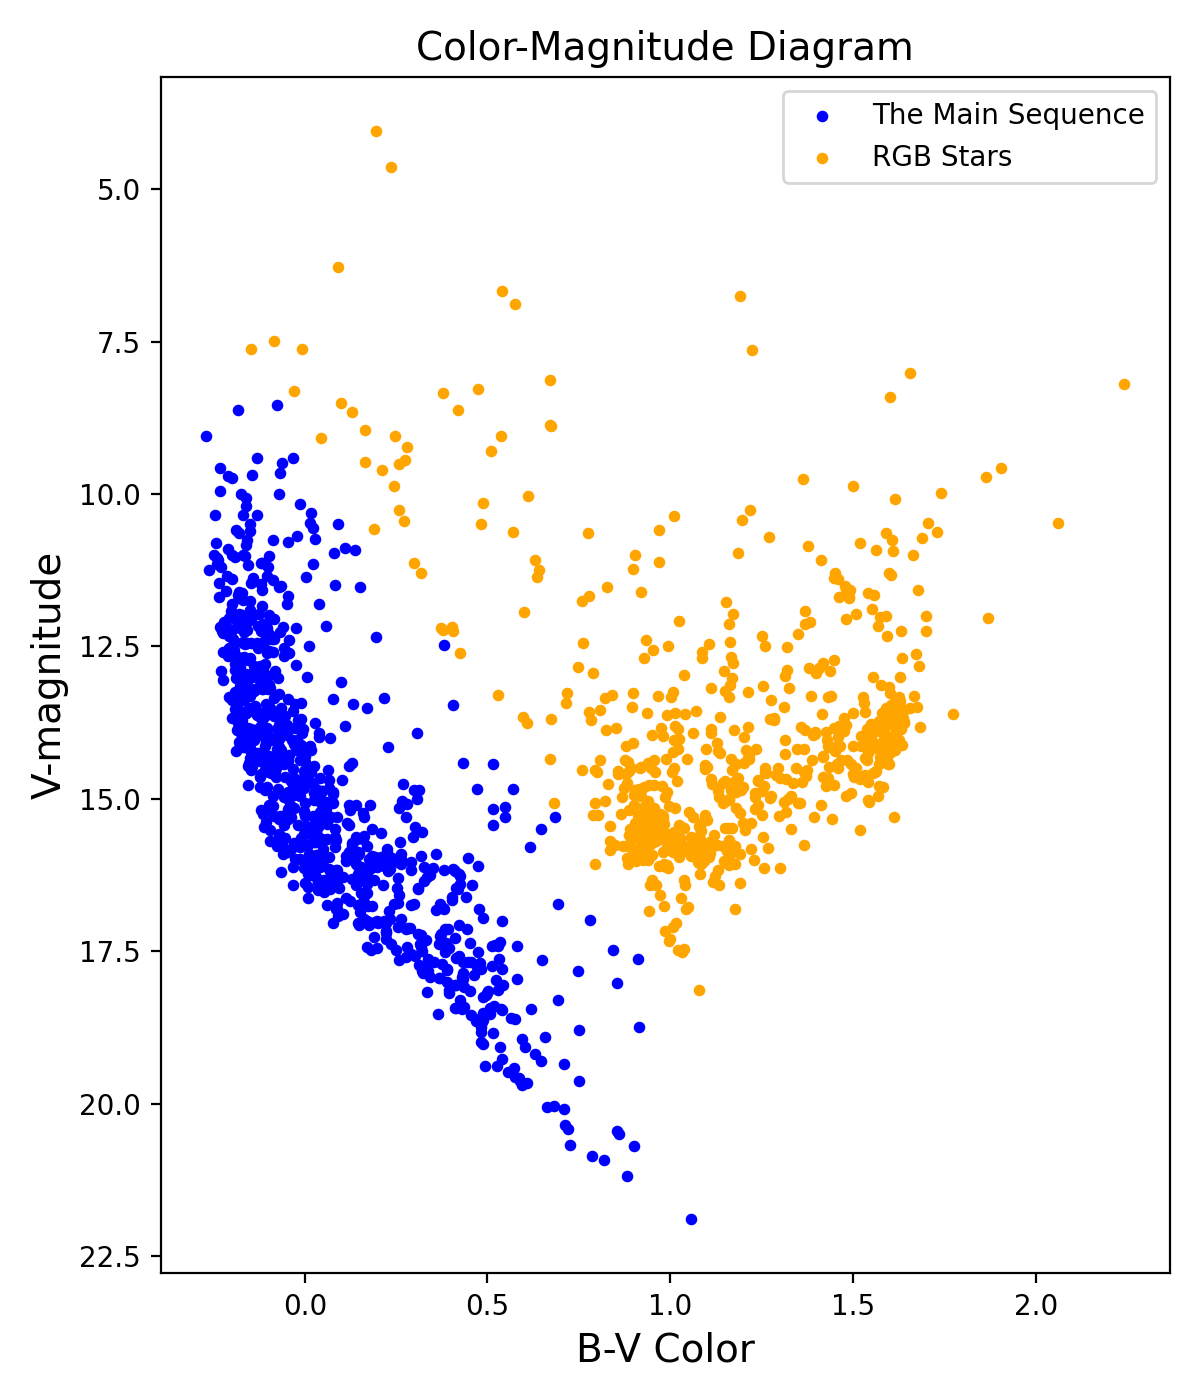
\includegraphics[width=8cm]{two_class.png}
    \caption{The color-magnitude diagram with classification}
    \label{class}
\end{figure}

\subsection*{(e)}
I plot the Hertsprung-Russell diagram (luminosity vs effective temperature) in 
Fig.\ref{class}
of the hipparcos-bright samples. 

\begin{figure}[htbp]
    \centering
    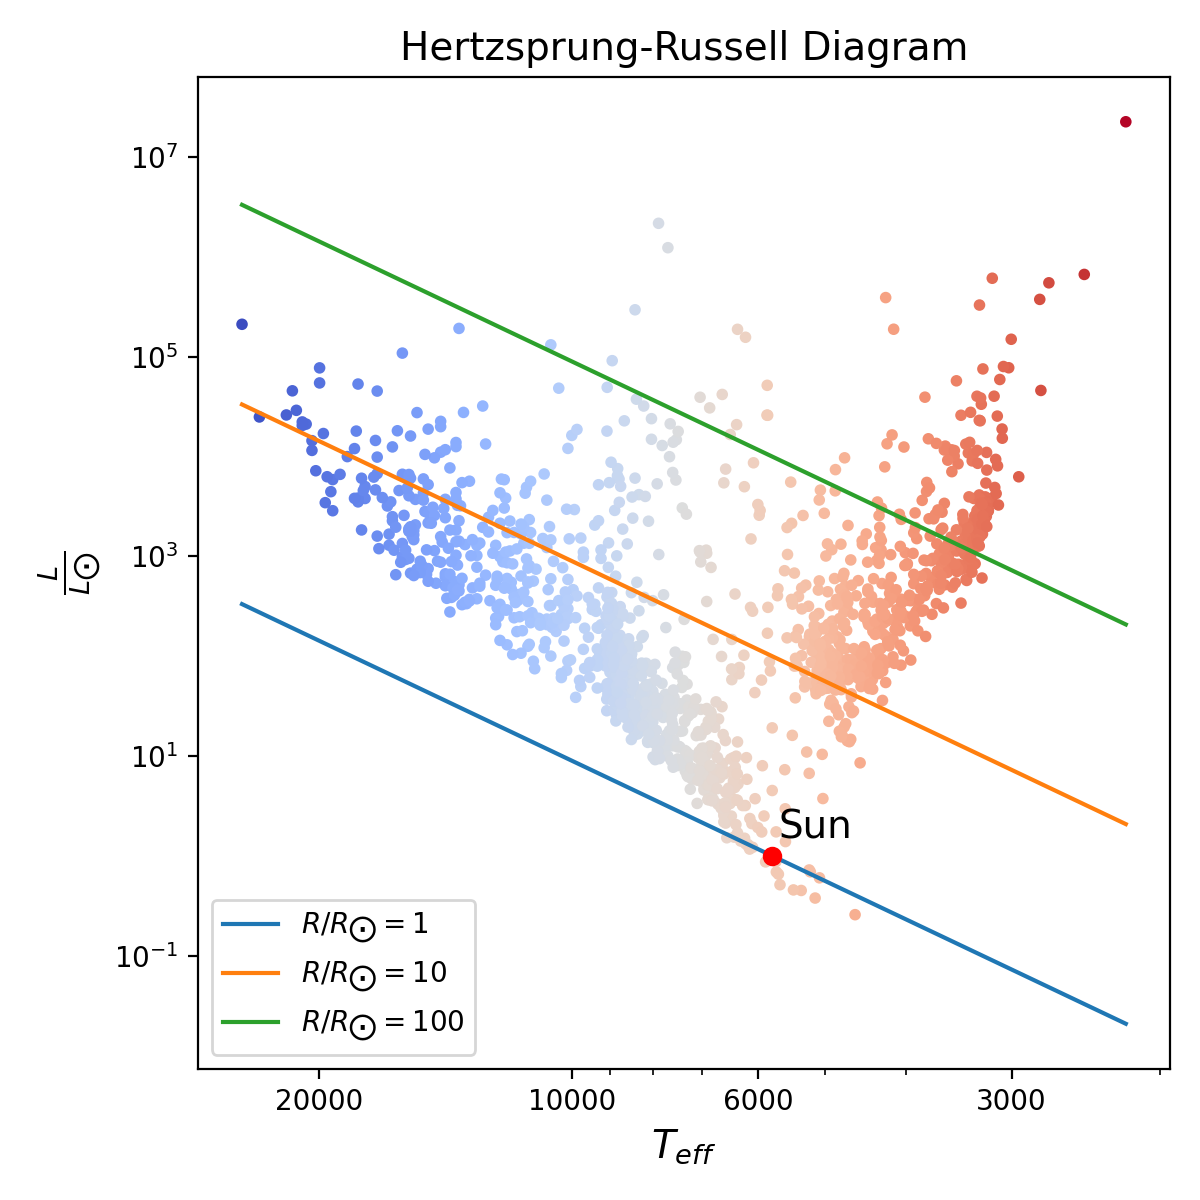
\includegraphics[width=10cm]{HR_diag.png}
    \caption{The Hertzsprung-Russell diagram of the hipparcos-bright samples}
    \label{class}
\end{figure}


\section*{\textbf{Exercise \uppercase\expandafter{\romannumeral1}.3 Transits}}
\subsection*{(a)}
We assume a circular orbit and uniform random probability distribution of orbital revolution axes on the unit sphere.
\begin{figure}[htbp]
    \centering
    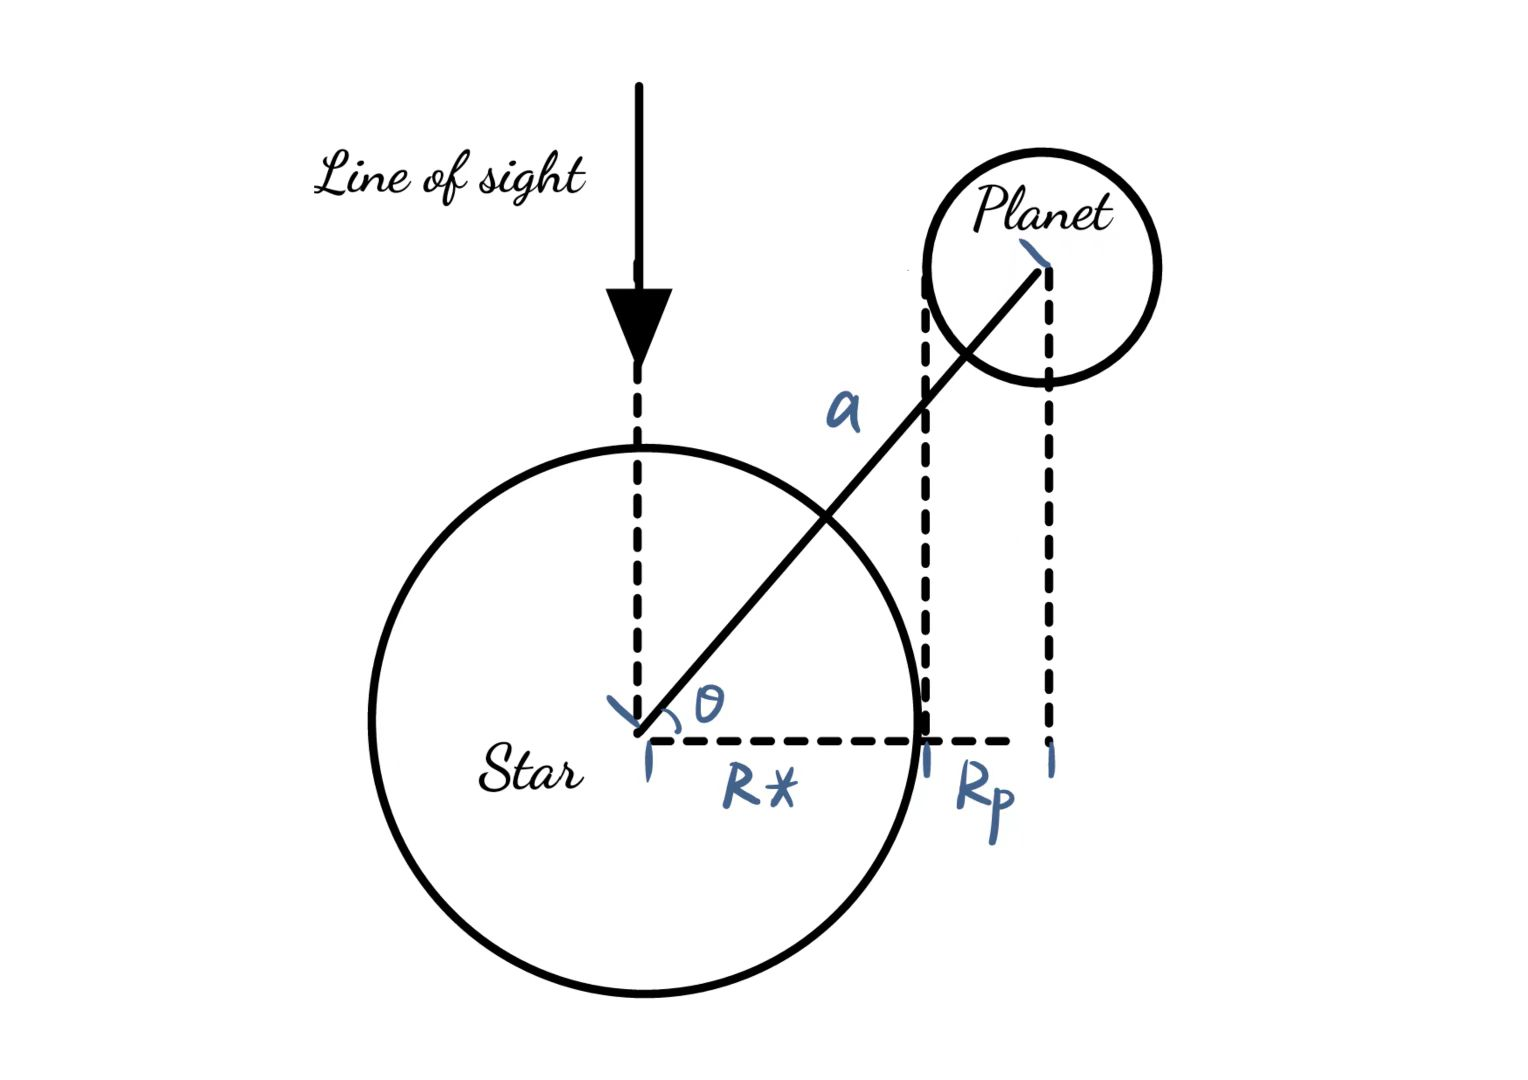
\includegraphics[width=12cm]{orbit.jpg}
    \caption{The orbit demenstration of a critical situation}
    \label{orbit}
\end{figure}

The probability of the transit not being observed by us is the fraction of 
the solid angle expanded by $\theta_0$ in Fig.\ref{orbit} and $2\pi$ (the solid angle of the half hemisphere):
\begin{align}
    \cos \theta_0 &= \frac{R_{\star}+R_\text{p}}{a} \\
    P_{\text{not-trans-orbit}} &= \frac{\int_{0}^{\theta_0}  \sin\theta \text{d}\theta \int_{0}^{2\pi} \text{d}\phi}{2 \pi}
                    = 1-\cos \theta_0
\end{align}
Therefore, the probability that a planet will transit at some point in its orbit is:
\begin{equation}
    P_{\text{trans-orbit}} = 1 - P_{\text{not-trans-orbit}} = \cos \theta_0 = \frac{R_{\star} + R_{\text{p}}}{a}
\end{equation}

\subsection*{(b)}
\begin{figure}[htbp]
    \centering
    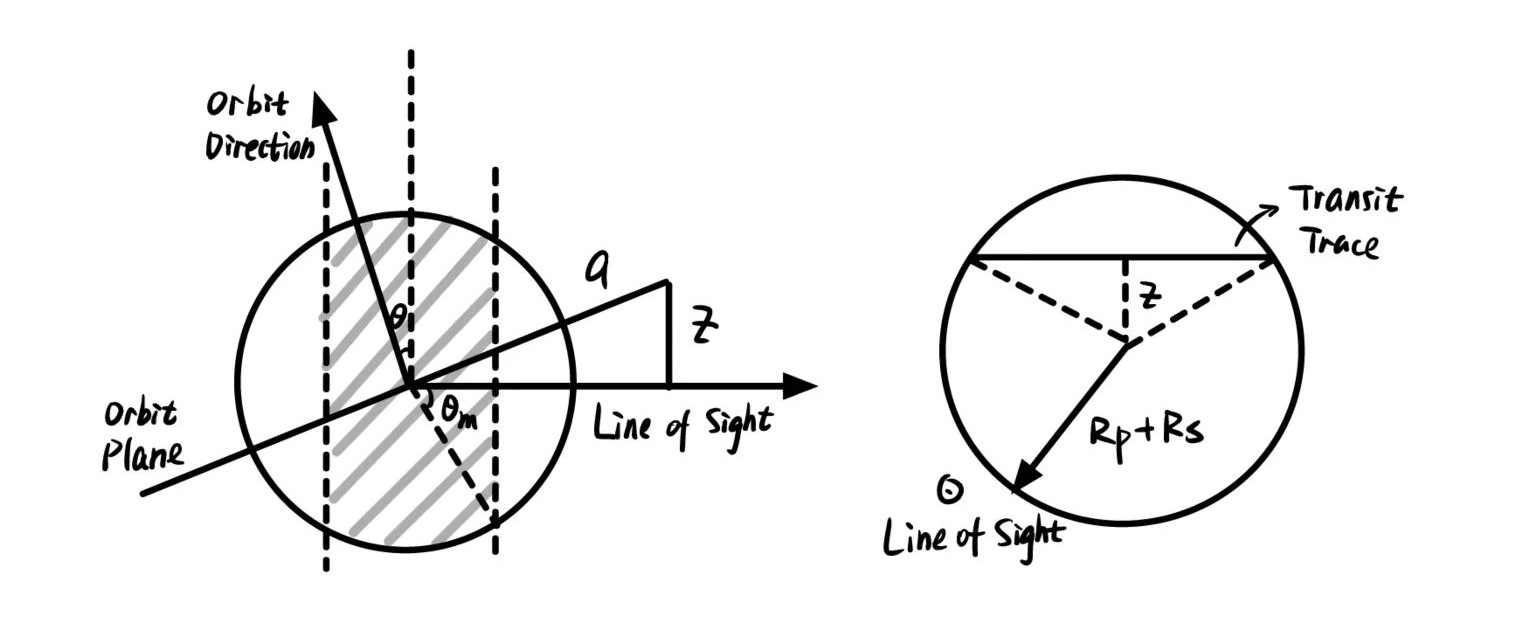
\includegraphics[width=14cm]{trainsit.jpg}
    \caption{The transit configuration}
    \label{transit}
\end{figure}
The side view of the planet transit is given in Fig.\ref{transit}, and only the planets whose 
orbital direction are in the shaded region can transit. From the geometry and the above problem(a) 
we can get that:
\begin{align*}
    \sin\theta_m & = \frac{R_{\text{p}} + R_{\star}}{a} \\
    z &= a \sin \theta
\end{align*}
As shown in Fig. , the length of the transit path $\Delta l$ can be approximated as:
\begin{equation}
    \Delta l  =2\sqrt{(R_{\text{p}} + R_{\star})^2 - z^2} = 2(R_{\text{p}} + R_{\star}) \sqrt{1 - (\frac{a \sin \theta}{R_{\text{p}} + R_{\star}})^2}
\end{equation}
The ratio of the transit duration and the orbital period is:
\begin{equation} 
    \frac{\Delta t}{T} = \frac{\Delta l}{2\pi a} = \frac{1}{\pi} \frac{R_{\text{p}} + R_{\star}}{a} \sqrt{1 - (\frac{a \sin \theta}{R_{\text{p}} + R_{\star}})^2}
\end{equation}
The fraction of possible orbits in the range $(\theta, \text{d}\theta)$ is $\frac{2\pi \cos \theta \text{d}\theta}{4 \pi} = \frac{1}{2}\cos \theta \text{d}\theta$,
so the probability of current transits can be written as:
\begin{align*}
    P &= \int_{-\theta_m}^{\theta_m} P_{\text{trans-orbit}}  \cdot \frac{\Delta t}{T} \cdot \frac{1}{2}\cos \theta \text{d}\theta  \\
     & = \frac{1}{2\pi} (\frac{R_{\text{p}} + R_{\star}}{a})^2 \int_{-\theta_m}^{\theta_m} \sqrt{1 - (\frac{\sin \theta}{\sin \theta_m})^2} \text{d} (\sin \theta) \\
     & = \frac{1}{4} (\frac{R_{\text{p}} + R_{\star}}{a})^2
\end{align*}

\subsection*{(c)}
Assuming that all of the $n = 100,000$ stars harbor such an Earth-like planet, 
so $R_{\star} = R_{\bigodot} = 7 \times 10^{10} \ \text{cm}$, 
$R_\text{p} = R_{\bigoplus } = 6.4 \times 10^{8} \ \text{cm}$ and 
$a = 1\ \text{AU} = 1.5 \times 10^{13} \ \text{cm}$.
Pluge into the equation (5) and we can get the number $N$
of the planets that will eventually show a transit is:
\begin{equation}
    N = P_{\text{trans-orbit}} \ n  = \frac{R_{\bigodot} + R_{\bigoplus}}{a} \ n \approx 471 
\end{equation}

\subsection*{(d)}
The maximum percentage change $\Delta$ in brightness 
of an Earth-like planet is:
\begin{equation}
    \Delta = \frac{\Delta F}{F} = \frac{\pi R_\text{P}^2}{\pi R_\star^2}
     = \frac{R_{\bigoplus}^2}{R_{\bigodot}^2}
     = 0.01 \%
\end{equation}
The relation between the magnitude $m$ and the flux $F$
is :
\begin{equation}
    m = -2.5 \log F + \text{const}
\end{equation}
Take derivatives on both sides and we get:
\begin{equation}
    \Delta m = -\frac{2.5}{\ln (10)} \frac{\Delta F}{F} \approx -1.086 \Delta = -1.086 \times 10^{-4}
\end{equation}
Therefore, the drop in magnitude is $\Delta m = -1.086 \times 10^{-4}$.

\subsection*{(e)}
I think Bernie is right. The white dwarf is as bright as the host star, so 
the white dwarf will not cause a dip in the their joint brightness when it orbits before the host star.
However, when the white dwarf orbits behind the host star, light emitted 
by the white dwarf will be blocked by the host star, resulting in a dip in their 
joint brightness, which is very similar to a transit signal. This effect 
is shown in Fig.\ref{binary}. In fact, eclipsing binary systems like 
this make up most of the falses positives in trasit planet detections.
\begin{figure}[htbp]
    \centering
    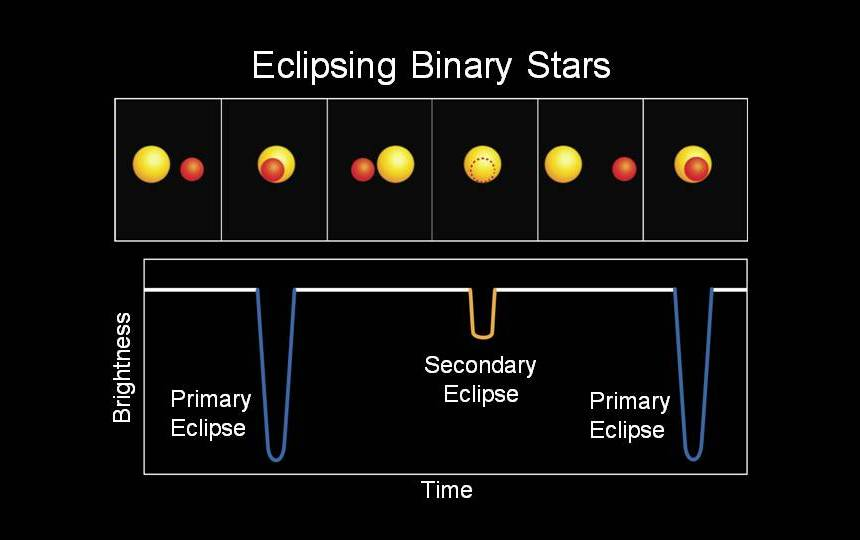
\includegraphics[width=12cm]{bianry.jpg}
    \caption{The orbit and light curve of en eclipsing bianry, credit: Wikimedia, NASA}
    \label{binary}
\end{figure}

\subsection*{(f)}
The radial-velocity amplitude $v_{\star}$ can be calculated from the following equations:
\begin{align}
    m_{\star} v_{\star} &= m_\text{p} v_\text{p} \\
    G(m_{\star} + m_\text{p}) &= \frac{4\pi^2 a^3}{P^2}
\end{align}
We notice that $vP = 2\pi a$, where $v = v_{\star}+v_\text{p}$, 
so we can cancel $P$ and $v_\text{p}$:
\begin{align*}
    & G(m_{\star} + m_\text{p}) = a (v_\star + \frac{m_{\star}v_{\star}}{m_\text{p}})^2 \\
    & v_\star = \frac{m_{\text{p}}}{m_{\text{p}}+m_\star} \sqrt{\frac{G(m_{\star} + m_\text{p})}{a}}
\end{align*}

For an Earth-like planet, we can get that $v_\star = 8.95 \ \text{cm} \ \text{s}^{-1}$;
for a white dwarf companion, we can get that $v_\star = 2106.12 \ \text{km}\  \text{s}^{-1}$.

\subsection*{(g)}
Due to the huge radial velocity amplitude of a white dwarf, we can rule out that 
the transiting body is a white dwarf by tanking an RV measurement.

\subsection*{(h)}
The precision of the current RV measurements is too low to detect 
the extreme small radial velocity amplitude of an Earth-like planet.
Therefore it is not useful to ensure that the transiting body is an Earth-mass planet using RV measurement.


\section*{\textbf{Exercise \uppercase\expandafter{\romannumeral1}.4  Microlensing}}
\subsection*{(a)}
Set the origin of $x$ axis at the periapsis of the trajectory, and denote the periapsis-passing time as $t=0$. At any time $t$, the $y$ component of the equation of motion is given by:
\begin{equation}
    \frac{\mathrm{d}v_y}{\mathrm{d}t}=\frac{GM}{b^2+x^2}=\frac{GM}{b^2+(vt)^2}.
\end{equation}
The above equation can be integrated directly and gives:
\begin{equation}
        v_y=\int_0^{v_y}\mathrm{d}v'_y=\int_{-\infty}^\infty\frac{GM}{b^2+(vt)^2}\mathrm{d}t=\frac{GM}{bv}\int_{-\infty}^\infty\frac{GM}{1+u^2}\mathrm{d}u=\frac{\pi GM}{bv}.
\end{equation}\\

\subsection*{(b)}
The scattering angle can easily be derived by:
\begin{equation}
    \psi\approx\frac{v_y}{v_x}=\frac{\pi GM}{bv^2}.
\end{equation}

\subsection*{(c)}
Assume that we have a source object at distance $d_s$ from the observer, and a lens object at distance $d_l<d_s$. We further assume that these two objects seen from the observer are aligned. Now we have the following geometric relation
\begin{equation}
    \psi(d_s-d_l)=\theta_\mathrm{E}d_s
\end{equation}
and
\begin{equation}
    b=\theta_\mathrm{E}d_l.
\end{equation}
Therefore we have:
\begin{equation}
    \frac{\pi GM}{\theta_\mathrm{E}d_l c^2}(d_s-d_l)=\theta_\mathrm{E}d_s.
\end{equation}
And it turns out to be:
\begin{equation}
    \theta_\mathrm{E}=\sqrt{\frac{\pi GM}{c^2}\frac{d_s-d_l}{d_s d_l}}.
\end{equation}

\subsection*{(d)}
The Einstein ring can be calculated as:
\begin{equation}
    \theta_E = \sqrt{\frac{4GM_{\text{L}}}{c^2} \frac{d_{\text{s}} - d_{\text{l}}}{d_{\text{l}}d_{\text{s}}}}
\end{equation}
Pluge in the values and we can get:
\begin{equation*}
    \theta_{\text{E}} = 3.46 \times 10^{-9} \ \text{radian} = 0.713 \ \text{mas}
\end{equation*}
The Einstein ring radius in the lens plane $r_{\text{lE}}$ is:
\begin{equation*}
    r_{\text{lE}} = \theta_{\text{E}} d_{\text{l}} = 2.854 \ \text{au}
\end{equation*}

The Einstein ring radius in the source plane $r_{\text{sE}}$ is:
\begin{equation*}
    r_{\text{sE}} = \theta_{\text{E}} d_{\text{s}} = 5.708 \ \text{au}
\end{equation*}

\subsection*{(e)}
The magnification is the same when $\beta = +/-\theta_{\text{E}}$, so we only need to 
calculate one situation. When $\beta = \theta_{\text{E}}$, the image $\theta$ satisfies
\begin{equation}
    \theta_\text{E} = \theta - \frac{\theta_{\text{E}}^2}{\theta}
\end{equation}
The two solutions to the above equation is:
\begin{align*}
    \theta_1 = 0.118 \theta_{\text{E}} \\
    \theta_2 = -2.118 \theta_{\text{E}} \\
\end{align*}
The magnification factor $m$ can be caldulated:
\begin{equation}
    m = \sum_{i = 1}^{2} \frac{\theta_i^4}{\theta_i^4 - \theta_{\text{E}}^4} = 1.052
\end{equation}
The source will be brighter in magnitude by $2.5\times \log_{10} m = 0.055$.

\subsection*{(f)}
From (e), we can see that when the source cross the 
Einstein ring, it is slightly magnified. Therefore, 
from the figure we can get that the duration of the Einstein 
ring crossing time is:
\begin{equation}
    t_{\text{E, cross, star}} = 8725 - 8650 = 75 \ \text{days}
\end{equation}

\subsection*{(g)}
Assuming that the proper motion speed between the source 
and the lens is the same during the microlensing event
and the caustic of the planet and the star does not affect each other
 very much (still perserve the Einstein ring shape), 
the mass ratio of the planet and the host star 
is proportional to the square root of the Einstein ring 
crossing time.
\begin{equation}
    \frac{m_{\text{p}}}{m_{\star}} = (\frac{\theta_{\text{E, planet}}}{\theta_{\text{E, star}}})^2 = (\frac{t_{\text{E, cross, planet}}}{t_{\text{E, cross, star}}})^2
\end{equation}
If $m_{\star} = 0.5 M_{\bigodot}$, then the mass of the planet is:
\begin{equation}
    m_{\text{p}} = m_\star (\frac{t_{\text{E, cross, planet}}}{t_{\text{E, cross, star}}})^2 = 1.85 \ M_{\bigoplus}
\end{equation}

\end{document}
